\section{Hardware}
Das Endprodukt setzt sich hauptsächlich aus dem Melde- und Sensor-Print zusammen. Die Anforderungen der Prints ist es, eine Datenübertragung von den einzelnen Solarpanels über eine Powerline zu einer Zentrale zu gewährleisten. Zudem muss der Sensorprint kompakt und an jedem Pannel montierbar sein.

In den nachfolgenden Kapiteln werden alle Teilschaltungen beschrieben um einen möglichen Nachbau zu erleichtern.

\subsection{Sensorprint}


Jedes Solarpanel wird mit einem Sensorprint auf der Rückseite des Panels bestückt. Der Sensorprint hat eine Grösse von 6 x 6cm und kann somit optimal in die vorgesehene Halterung auf der Rückseite des Panels eingebaut werden. Als Vorlage für die grösse der Halterung, wurde das Austellemodell im Labor in betracht gezogen.

Der Aufbau des Sensorprints besteht aus einem Mikrocontroller, einem Powerline-Transceiver, einem ADC-Converter und einer 12V-Speisung. Seine Aufgabe ist die Spannungswerte des Solarpanels einzulesen, diese zu verarbeiten und die Informationen über die Powerline an den Meldeprint zu übermitteln. Dieses Konzept veranschaulicht die Abbildung 2.

\begin{figure}[h]
\centering
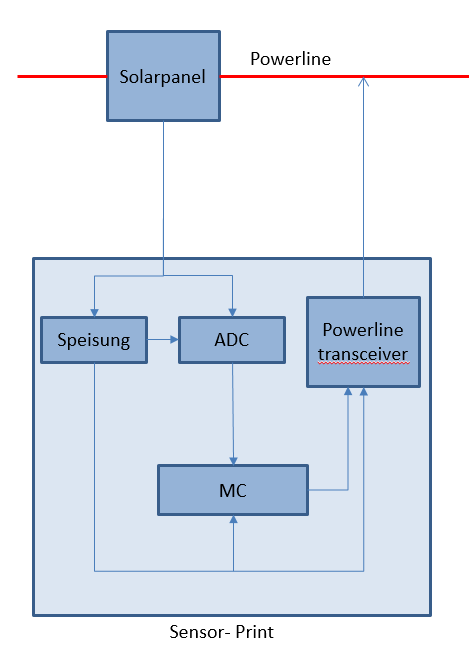
\includegraphics[width=0.5\textwidth]{konzept_sensor}
\caption{Grobkonzept des Sensorprints}
\end{figure}

Eine grobe Übersicht über den Aufbau und das Zusammenspiel der einzelnen Komponenten ist auf Abbildung 2 zu sehen.



\subsubsection{Speisung}
Die Speisung des Sensorprints erfolgt über einen LM-2594-DC/DC-Regulator. Das Bauteil wurde gewählt, weil es einen Spannungsbereich gemäss unseren Anforderungen am Eingang gewährleistet.

Eine variable Eingangsspannung von 12V-60V vom Solarpanel wird am Eingang detektiert. Der DC/DC-Regulator regelt diese Eingangsspannung mit Hilfe eines Schaltreglers auf eine feste 12V DC Spannung am Ausgang. Diese Spannung gewährleistet die Versorgung des Powerline Transceivers. Die restlichen Elemente werden mit 5V (VDC) gespiesen.

Die 5V DC Spannung wurde anders als geplant realisiert. Auf dem Print war nur Platz für eine Speiseschaltung vorgesehen, darum musste die 5V-Spannung über den 5V-Ausgang des Powerline Transceivers realisiert werden. Da nur eine mittlere Leistung von maximal 100mW auf dem Sensorprint vorhanden ist, ist diese Beschaltung realisierbar.

In der nachfolgenden Abbildung 3 ist die Beschaltung der 12V Speisung (VCC) ersichtlich.


\begin{figure}[h]
\centering
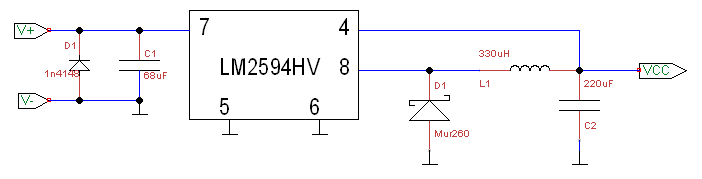
\includegraphics[width=1\textwidth]{speisung_sensor}
\caption{Beschaltung der 12V-Speisung}
\end{figure}

Die ersichtlichen Bauteile auf Abbildung 3wurden anhand der Datenblattvorgaben des LM2594 \cite{DCDC_Regulator_LM2594} ausgewählt.

\clearpage
\subsubsection{Spannungsmessung}
Die Spannungsmessung erfolgt über einen Analog-Digital-Converter (MCP 3202). Am Analog-Input (Ch0) des ADC's wird die Spannung des Solarpanels eingelesen. Da nur 0V-5V eingelesen werden können, wird die Spannung mit einem Spannungsteiler entsprechend skaliert. Der analoge Wert wird vom ADC in einen binären 12-Bit-Wert (0V = 0000 0000 0000, 5V = 1111 1111 1111) umgewandelt und über den digitalen Output (Dout) zum Mikrocontroller übertragen. Ein 12 Bit ADC wurde gewählt, um die Genauigkeit der Spannungsmessung von 0.1V zwischen 12V und 60V zu gewährleisten. MIt dem 12 Bit ADC können wir eine Messgenaugkeit von 1.25mV gewährleisten. Auf Abbildung 4 ist die Innenarchitektur des ADC's sichtbat

\begin{figure}[h]
\centering
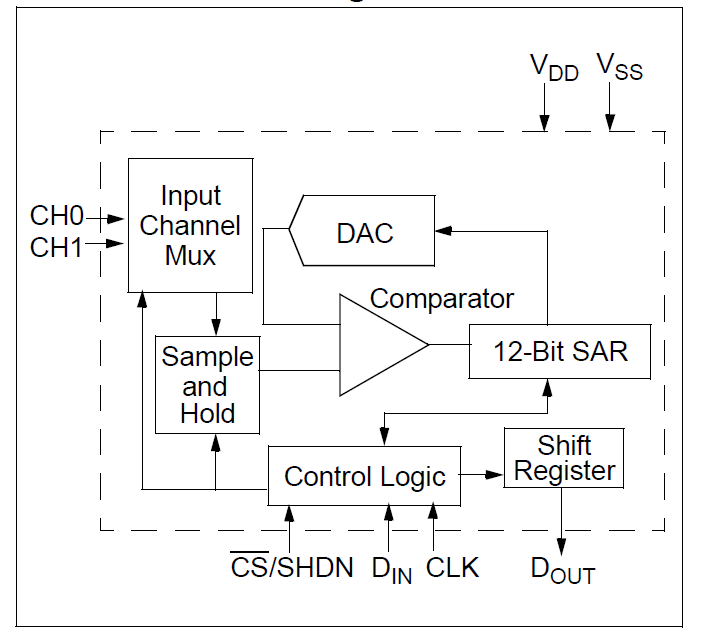
\includegraphics[width=0.5\textwidth]{adc}
\caption{Aufbau des ADC's \cite{Datasheet_adc}}
\end{figure}

Um den Ablauf der Umwandlung von einem analogen Spannungswert auf einen digitalen Binärwert besser nachvollziehen zu können, ist auf Abbildung 4 die innere Architektur des Analog-Digital-Converters ersichtlich.

\
\

\subsubsection{Mikrocontroller}
Als zentrale Steuereinheit des Sensorprints wurde ein Arduino-Nano-Board mit einem Atmega-328-Chip ausgewählt. Dieses Board wurde gewählt, weil in vorgängigen Projekten bereits damit gearbeitet wurde. Zudem können unsere Anforderungen mit der vorhandenen Leistung und Speicherkapazität des Mikrocontrollers problemlos realisiert werden. Als Verbesserung könnte man den Atmega 328 und seine Grundbeschaltung direkt auf den Print bestücken. Somit könnte man Platz sparen und den Print noch komprimierter herstellen.

Die Aufgabe des Mikrocontrollers auf dem Sensorprint beruht im Allgemeinen darauf, die Verbindung zwischen dem ADC und dem Powerline Transceiver herzustellen. Die Verbindung zwischen Mikrocontroller und ADC funktioniert mit SPI-Kommunikation. Diejenige zum Powerline Transceiver wird über UART-Kommunikation hergestellt. Detailiertere Informationen zur Kommunikation der einzelnen Elemente untereinander sind im Abschnitt \ref{Software_sensorprint} unter Software zufinden.


\clearpage

\subsubsection{Adressierung}
Um das Panel identifizeren zu können, wurde Hardware basierend eine binäre Adressierung vorgesehen. Diese erfolgt über einen binären 8-Bit-Wert, welcher mit Dip-Switch Schaltern eingestellt werden kann. Dieser wird parallel an 8 digitalen-Eingängen am Mikrocontroller eingelesen. Wenn ein Schalter gedrückt wird, gelangt 5V (=1) an den Eingang des Mikrocontrollers.

Die Beschaltung der Schalter ist auf Abbildung 5 ersichtlich.

\begin{figure}[h]
\centering
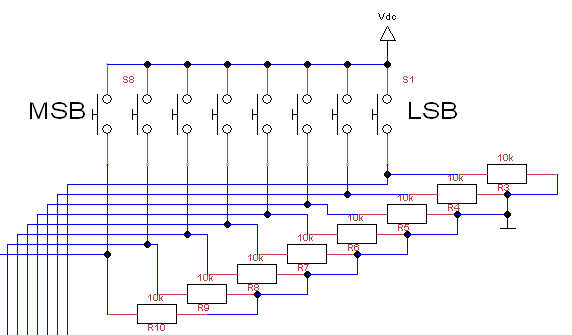
\includegraphics[width=1\textwidth]{adressierung}
\caption{Beschaltung der Schalter}
\end{figure}

 Wenn der Schalter offen ist, gelangt 0V (=0) mittels 10kOhm pull-down-Widerständen an den Eingang. Mit 8 Schaltern können somit 256 Pannels adressiert werden.
 
\clearpage

\subsubsection{Transceiver}
Für die Modelierung der Daten der Solarpanels, benutzen wir einen ST7540-Powerline-Transceiver. Dieses Bauteil wurde gewählt, weil 8 Übertragungsfrequenzen bereits einprogrammiert sind, sowie 4 Baudraten. Der Transceiver empfängt vom Mikrocontroller über den TxD Eingang ein Signal. Dieses Signal wird intern mit frequency shift keying (FSK) modeliert. Als Übertragungsfrequenz wurde 132.5kHz gewählt. Das modelierte Signal wird an den Ausgang übertragen und mittels induktiver Einkopplung auf die Powerline eingekoppelt. Die Einkopplung erfolgt mittels einem Draht, welcher um einen Feritkern gewickelt wurde. Dieses Zusammenspiel erzeugt eine Induktion und ermöglicht somit die Einkopplung auf die Powerline. Dieser Prozess ist die Kernaufgabe dieses Projektes und wird im Abschnitt\ref{sec::Theorie} genauer erläutert. Auf Abbildung 6 ist die Beschaltung des Powerline Transceivers ersichtlich.

\begin{figure}[h]
\centering
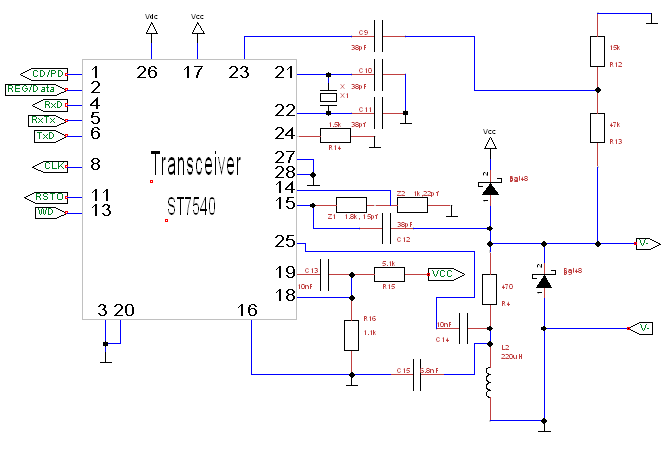
\includegraphics[width=0.7\textwidth]{transceiver}
\caption{Beschaltung des Transceiver}
\end{figure}

Auf der linken Seite des Transceivers, in Abbildung 6, sind die Ein-und-Ausgänge für die UART-Kommunikation vorhanden. Wie bereits im Abschnitt 3.1.1 Speisung erwähnt wurde, gewährleistet der Powerline Transceiver die 5V-Speisung mit Pin 26.
Bei ''V-'' erfolgt die Einkopplung des FSK modulierten Signals auf die Powerline. Alle vorhandenen Bauteile dieser Beschaltung wurden anhand der Datenblattinformationen des ST7540 berechnet, dimensioniert und ausgewählt.
